\documentclass[conference]{IEEEtran}


%\usepackage{geometry}
\usepackage{optidef}
\usepackage{balance}
\usepackage{amsmath}
\usepackage{amssymb}
\usepackage{amsthm}
\usepackage{times}
\usepackage{helvet}
\usepackage{courier}
\usepackage{graphicx}
\usepackage{subfigure}
\usepackage{mdwmath}
\usepackage{mdwtab}
\usepackage{amssymb}
\usepackage{booktabs}
\usepackage{algorithm}
\usepackage{pifont}
\usepackage{algpseudocode}
\usepackage{balance}
\usepackage{bm}
%\usepackage{ulem}
\usepackage[normalem]{ulem}
\usepackage{array}
\usepackage{balance}
\usepackage{multirow}
\usepackage{multicol}
\usepackage{threeparttable}
\frenchspacing
\usepackage[marginal]{footmisc}
\usepackage{extarrows}
\usepackage{natbib}

%add the command initial
\algnewcommand\algorithmicInitial{\textbf{Initialize:}}
\algnewcommand\Initial{\item[\algorithmicInitial]}
\algnewcommand\algorithmicIterate{\textbf{Iterate:}}
\algnewcommand\Iterate{\item[\algorithmicIterate]}
\algnewcommand\algorithmicInput{\textbf{Input:}}
\algnewcommand\Input{\item[\algorithmicInput]}



\ifCLASSINFOpdf

\else

\fi



% correct bad hyphenation here
\hyphenation{op-tical net-works semi-conduc-tor}


\begin{document}
%
% paper title
% Titles are generally capitalized except for words such as a, an, and, as,
% at, but, by, for, in, nor, of, on, or, the, to and up, which are usually
% not capitalized unless they are the first or last word of the title.
% Linebreaks \\ can be used within to get better formatting as desired.
% Do not put math or special symbols in the title.
%\title{Bare Demo of IEEEtran.cls\\ for IEEE Conferences}
\title{Advanced Stochastic Optimization for PCA and PLS: Variance Reduction and Asynchronism}

% author names and affiliations
% use a multiple column layout for up to three different
% affiliations



\balance


\maketitle


\begin{abstract}
Principal Component Analysis(PCA) is a dimensionality reduction technique which extract the representative components of the data. Partial Least Squares(PLS) models the covariance structure between a pair of data matrices. Both of them are widely used in many areas and can be represented as a similar objective function. Deterministic methods like the full singular value decomposition (SVD) for these problems suffers from prohibitive computation cost in large-scale applications, while the stochastic or incremental algorithms fail to achieve a high accuracy. In this paper, we propose stochastic optimization methods with variance reduction to solve PCA and PLS, which ensure to obtain high accuracy solutions with enough computation cost and rapidly converge to an approximate optima with  few iterations. Moreover, we explore an asynchronous implement of stochastic optimization for the two problems. Extensive experiments illustrates the significant performance of our method.


\end{abstract}


\IEEEpeerreviewmaketitle



\section{Introduction}
\label{introduction}
Principal component analysis (PCA) is a popular dimensionality reduction technique widely used in many areas, such as machine learning, statistics, computer vision \citep{Stockman2001Computer}. The goal of PCA is to find the maximal (uncentered) variance $k$-dimensional subspace with respect to a $d \times n$ matrix $X = (\mathbf{x}_1, ... , \mathbf{x}_n)$. It is equivalent to solve the following optimization problem:
\begin{equation}
\label{pca-obj}
\begin{aligned}
& \underset{W}{\text{maximize}}
& & \mathrm{Trace}(W^{\top}(\frac{1}{n}\sum\limits_{i=1}^{n}\mathbf{x}_{i}{\mathbf{x}_i}^\top)W) \\
& \text{subject to}
& & W^{\top}W=I \\
%&&& X \succeq 0.
\end{aligned}
\end{equation}
The  $d\times k$ matrix $W$ is used to parameterize the subspace.
Partial least squares (PLS) \citep{Chiang2001Partial}, a ubiquitous method for bilinear factor analysis, is widely used in information retrieval \citep{Salton2003Information} and machine learning. It solves the following problem: given a dataset of $n$ samples including  two sets of features, 
%$x \in \mathbb{R}^{d_x}$ and $y \in \mathbb{R}^{d_y}$, respectively, 
the $d_x \times n$ matrix $X = (\mathbf{x}_1, ... , \mathbf{x}_n)$ and the $d_y \times n$ matrix $Y = (\mathbf{y}_1, ... , \mathbf{y}_n)$, what is the $k$-dimensional subspace that captures most of the covariance between the two views. 
The PLS problem can be expressed as:
\begin{equation}
\label{pls-obj}
\begin{aligned}
& \underset{U,V}{\text{maximize}}
& & \mathrm{Trace}(U^{\top}(\frac{1}{n}\sum\limits_{i=1}^{n}\mathbf{x}_{i}{\mathbf{y}_i}^\top)V) \\
& \text{subject to}
& & U^{\top}U = I, V^{\top}V=I \\
%&&& X \succeq 0.
\end{aligned}
\end{equation}

The pair of  matrices $U \in \mathbb{R}^{d_x \times k}$ and $V \in \mathbb{R}^{d_y \times k}$ are the solution of PLS. 
It is obvious that the objective functions of PCA and PLS are quite similar, and PCA is a special case of PLS, thus they can be solved through the same algorithms.
It is well known that the subspaces can be given by applying the singular value decomposition to the $d_x \times d_x$ covariance matrix $XX^\top$ for PCA and the $d_x \times d_y$ cross-covariance matrix $XY^\top$ for PLS. However, the exact singular value decomposition is infeasible for big-data scenarios as its required runtime is $O(\mathrm{min}(k^2d,kd^2))$ for a $k \times d$ matrix.
In recent years, studies on solving $k$-SVD have made many breakthroughs \citep{Bhojanapalli2014Tighter}\citep{Musco2015Randomized}\citep{Halko2010Finding},  becoming great options to solving such the covariance matrices. 
However, in this paper, we only focus on objective functions like problem (\ref{pca-obj}) and (\ref{pls-obj}), whose covariance matrix can be approximated by a random rank-1 $\mathbf{x}_{i}{\mathbf{y}_i}^\top$.
Standard deterministic approaches based on power iterations are accurate but require a full pass over the entire dataset, which is also expensive in the ``data laden" regime. Recently, stochastic optimization algorithms have developed a lot to deal with massive data.
The simplest stochastic algorithm for PCA and PLS are the stochastic power methods such as Oja algorithm \citep{Oja1982Simplified} and Hebbian algorithm \citep{Sanger1989Optimal}. Another straightforward approach is the incremental method \citep{Arora2014Stochastic}, which can be implemented efficiently. Besides, the online algorithms such as Matrix Stochastic Gradient(MSE) and Matrix Exponentiated Gradient(MEG) \citep{Arora2016Stochastic}\citep{Arora2013Stochastic} have been proposed, with great theoretical guarantee. In contrast to the deterministic algorithm, these algorithm randomly sample some examples to update the parameters, which performs much cheaper iterations. 
The drawback of stochastic algorithms is that the noise caused by stochastic sample means they converge sublinearly and have difficulty in obtaining a high-accuracy solution.
Recently,  Ohad Shamir made a breakthrough in \citep{Shamir2015Fast} by proposing VR-PCA, 
a novel algorithm for PCA problem, which is based on cheap stochastic iterations, yet converging linearly to obtain accuracy $\epsilon$. This algorithm combines the stochastic power method with the stochastic variance reduced gradient(SVRG) proposed in \citep{IEEE2013Accelerating}, shows better performance than the primal stochastic power method. Inspired by VR-PCA, we similarly apply the variance reduced stochastic algorithm to PLS and propose VR-PLS. Moreover, as SVRG-based algorithms require passing through the entire data as a ``Preparation Step" for generating the consequent variance reduced stochastic iterations at the beginning of each epoch, which is rather time-consuming. As a result, when using VR-PCA, the objective will not be optimized until at least $O(nd)$ runtime is consumed, thus it cannot be applied when computation resource is very limited. Inspired by another variance reduced stochastic gradient algorithm, i.e., SAGA\citep{Defazio2014SAGA}, we design two novel stochastic algorithms, VR-PCA+ and VR-PLS+, to solve PCA and PLS respectively. The SAGA-based algorithms are superior to SVRG-based algorithms in our experiments, and optimize the objective immediately without such ``Preparation step". Furthermore, since stochastic power method is intrinsically suitable for asynchronism, we design an asynchronous stochastic power method to utilize the multi-core systems.
In brief, our contributions are highlighted as follows:
\begin {itemize}
\item We extend the variance reduction technique to the stochastic optimization for partial least square, proposing the  VR-PLS algorithm, which is capable to achieve high accuracy solutions.
\item We introduce the SAGA algorithm into the optimization of PCA and PLS, resulting in two novel algorithms, VR-PCA+ and VR-PLS+.
\item We implement an asynchronous stochastic power method for PCA and PLS, which accelerates the convergence through multi-threads.
\item Extensive experiments demonstrate the effectiveness and efficiency of our proposed algorithms, which outperform their counterparts significantly on the convergence performance.
\end {itemize}

This paper is organized as follows: 
Section \ref{preliminaries} introduces the SVRG algorithm and SAGA algorithm. Section \ref{SVRG-based} presents the SVRG-based algorithm, i.e., VR-PCA and VR-PLS. Section  \ref{SAGA-based} presents the SAGA-based algorithm, i.e. , VR-PCA+ and VR-PLS+. Section \ref{ASGD} explores the asynchronous implement of stochastic power method. Section \ref{experiments} demonstrates the numerical results of our algorithms. Section \ref{discussion} concludes the strengths and weaknesses of our work and presents the future works.
%\section{Related work}
%\label{related work}

\section{Preliminaries}
\label{preliminaries}
 In this section we review the SVRG algorithm and SAGA algorithm. 
 As is shown in Algorithm \ref{SVRG}, there are two loops in SVRG. At the beginning of each outer loop (which is called an $epoch$), the entire dataset is computed and a batch gradient $\tilde{\mu}$ is achieved. In each inner loop, a stochastic gradient with lower variance is generated to update the parameters. The update rule is $\omega_{t} = \omega_{t-1} - \eta g_t$, while 
 $$g_t = \nabla f_{i_t}(\omega_{t}) - \nabla f_{i_t}(\tilde{\omega}_s)+\tilde{\mu}$$
 Note that the expectation of $\nabla f_{i_t}(\tilde{\omega}_s)$ over $i_t$ is $\tilde{\mu}$, and the expectation of $\nabla f_{i_t}(\omega_{t})$ over $i_t$ is $\nabla F(\omega_{t})$. We thus obtain 
 $$\mathbb{E}[\omega_{t+1} | \omega_{t}] = \omega_{t} - \eta\nabla F(\omega_{t})$$
 And the variance of $g_t$ is expected to be smaller than simply choosing $g_t=\nabla f_{i_t}(\omega_{t-1})$. At the end of each epoch, $\tilde{\omega}_{s+1}$ is updated based on the outputs of inner loop. Note there are two options for the update. SVRG with both the options have been theoretically proved to converge linearly, while SVRG with Option \uppercase\expandafter{\romannumeral1} performs better in practice. Thus we adopt Option \uppercase\expandafter{\romannumeral1} in this paper. 

Note that SVRG requires to compute a batch gradient at the start of each epoch, which is quite time-consuming. SAGA avoids the calculation of batch gradients, at the expense of some storage overhead. The algorithm has to store $\nabla f_{i}(\omega_{[i]})(i \in {1, ... , n})$, where $\omega_{[i]}$ denotes the latest iteration at which $\nabla f_i$ was computed. In each iteration, a random integer $j \in {1, ..., n}$ is chosen and the following stochastic vector is executed:
$$g_k = \nabla f_{j}(\omega_{k}) - \nabla f_{j}(\omega_{[j]}) + \frac{1}{n} \sum\limits_{i=1}^{n}\nabla f_{i}(\omega_{[i]})$$
Taking the expectation of $g_k$ over $j$, one again obtains that 
 $\mathbb{E}[g_k | \omega_t] = \nabla F(\omega_{t})$
 Therefore, $g_k$ is an unbiased gradient estimate, and has lower variance than stochastic gradients. 
 SAGA proved to also have a linear convergence rate, not requiring to compute batch gradients occasionally. Hence, SAGA often performs better than SVRG in practice. One important drawback of SAGA is the requirement of storing $n$ stochastic gradient vectors, which is infeasible in large-scale applications. However, fortunately, in many cases, $\nabla f_{j}$ is not necessary to be stored explicitly. For example, if the form of the component functions are $f_j(\omega_k) = \tilde{f}({\mathbf{x}_j}^{\top}\omega_k)$, one only need to store a scalar to construct the $\nabla f_j(\omega_k)$. In this paper, one important reason for applying SAGA to PCA and PLS is that both of them benefit from this character.
 
  \begin{algorithm}[t]
 	\caption{\textsc{SVRG}}
	\label{SVRG}
	\begin{algorithmic}[1]
	\Require the learning rate $\eta$,  the epoch size $m$, initial $\tilde{\omega}_0$
	\For {$s=0, 1, 2, ... $}
		\State $\tilde{\mu} = \frac{1}{n}\sum\limits_{i=1}^{n}\nabla f_{i}(\tilde{\omega}_{s})$
		\State $\omega_0 = \tilde{\omega}_s$
		%compute the batch gradient 
		\For {$t=0, 1, ..., m-1$}
			\State Randomly pick $i_t\in\{1, 2, ..., n\}$
			\State $\omega_{t+1} = \omega_{t} - \eta(\nabla f_{i_t}(\omega_{t}) - \nabla f_{i_t}(\tilde{\omega}_s)+\tilde{\mu})$
		\EndFor
		\State \textbf{Option \uppercase\expandafter{\romannumeral1}:} $\tilde{\omega}_{s+1} = \omega_{m}$
		\State \textbf{Option \uppercase\expandafter{\romannumeral2}:} $\tilde{\omega}_{s+1} = \omega_{t}$ for randomly chosen $t \in \{0, ... ,m - 1\}$ 
	\EndFor
	\end{algorithmic}
\end{algorithm}


\begin{algorithm}[t]
	\caption{\textsc{SAGA}}
	\label{SAGA}
	\begin{algorithmic}[1]
	\Require the learning rate $\eta$,  initial $\omega_0$
	\For {$i=1, 2 , ... n$}
		\State $\nabla f_{i}(\omega_{[i]}) = \nabla f_{i}(\omega_{0})$
	\EndFor
	\For {$k=1, 2, 3, ...$}
		\State Randomly pick $j\in{1, 2, ..., n}$
		\State $g_k = \nabla f_{j}(\omega_{k}) - \nabla f_{j}(\omega_{[j]}) + \frac{1}{n} \sum\limits_{i=1}^{n}\nabla f_{i}(\omega_{[i]})$
		\State $\nabla f_{j}(\omega_{[j]}) = \nabla f_{j}(\omega_{k})$
		\State $\omega_{k+1} = \omega_{k} - \eta g_k$
		
	\EndFor 
	\end{algorithmic}

\end{algorithm}

 
 \section{SVRG-based algorithm}
 \label{SVRG-based}
 In this section we present the SVRG-based algorithms for PCA and PLS. We first review the VR-PCA algorithm proposed in \citep{Shamir2015A}, and then analogically propose VR-PLS, a variance reduced stochastic algorithm for PLS.
 \subsection{VR-PCA}
 Stochastic gradient descent (SGD) is a simple but efficient optimization method, which is commonly used in a variety of unconstrained optimization problems. Although the objective function of PCA is constraint, the stochastic gradient descent still works. The variant of SGD, called stochastic power method, was proposed in \citep{Arora2014Stochastic}. It takes the following update rule in each iteration:
 \begin{equation}
 \label{sgd-pca}
 W_{t+1} = P_{orth}(W_{t} - \eta_t \mathbf{x}_{t}\mathbf{x}_{t}^{\top}W_{t})
 \end{equation}
 Notice that the runtime of calculating $\mathbf{x}_{t}\mathbf{x}_{t}^{\top}W$ is only $O(kd)$, which is rather cheap. $P_{orth}$ indicates the normalization step such as  Gram-Schmidt procedure to ensure the orthogonal condition $W^{\top}W=I$. The orthogonalization procedure requires runtime $O(k^2d)$, but may be performed infrequently without affecting the correctness of the algorithm, thus its computational cost can be ignored.
 In our implements, we adopt a more stable transformation proposed in \citep{Shamir2015Fast} as follows:
 \begin{equation}
 \label{orthogonalization}
 W_t = \hat{W_t}(\hat{W_t}^{\top}\hat{W_t})^{-1/2}
 \end{equation}
 The $\hat{W_t}$ is the output of iteration $t$ without normalization.
 For simplicity, we still use SGD to represent the stochastic power method in this paper.
 Despite the fact that the SGD algorithm for PCA converges rapidly to a neighbourhood of optima, it fluctuates near the optima and fails to converge. Hence, the a fast stochastic algorithm called VR-PCA was proposed in \citep{Shamir2015A}, inspired by the SVRG algorithm. As is shown in Algorithm \ref{VR-PCA}, VR-PCA consists of several epochs, and each epoch includes a batch gradient computation and $m$ cheap stochastic iterations. The variance reduced stochastic iteration is similar to that of SVRG, can be express as
 \begin{equation}
 \label{vr-sgd-pca}
 W_{t+1} = P_{orth}(W_{t} - \eta(\mathbf{x}_{i_t}\mathbf{x}_{i_t}^{\top}W_{t}- \mathbf{x}_{i_t}\mathbf{x}_{i_t}^{\top}\tilde{W}_{s}+\tilde{\mu}))
 \end{equation}
  As computing the matrix-vector multiplication takes the main cost of one iteration, that Equation \ref{vr-sgd-pca} can be reformed as 
 \begin{equation}
 \label{vr-sgd-pca2}
 W_{t+1} = P_{orth}(W_{t} - \eta(\mathbf{x}_{i_t}\mathbf{x}_{i_t}^{\top}(W_{t}-\tilde{W}_{s})+\tilde{\mu}))
 \end{equation}
 Note that the computation cost of \ref{vr-sgd-pca2} is the half of that of \ref{vr-sgd-pca}.
 Both theory and experiments in \citep{Shamir2015A} demonstrate the linear convergence of VR-PCA.
 
 \subsection{VR-PLS}
 It is natural to extend the variance reduced SGD algorithm of PCA to PLS as their objective functions have the analogous structure. As is shown in Algorithm \ref{VR-PLS}, the difference is that PLS chooses a pair of samples $\mathbf{x}_t, \mathbf{y}_t$ in each iteration and we should compute gradients with regards to $U$ and $V$ respectively. Thus the stochastic gradient update consists two parts: 
 \begin{equation}
 \begin{split}
 U_{t+1} = P_{orth}(U_{t} - \eta(\mathbf{x}_{i_t} {\mathbf{y}_{i_t}}^{\top}(V_t - \tilde{V}_s) + \tilde{\mu}_U))\\
 V_{t+1} = P_{orth}(V_{t} - \eta(\mathbf{y}_{i_t} {\mathbf{x}_{i_t}}^{\top}(U_t - \tilde{U}_s) + \tilde{\mu}_V))
 \end{split}
 \end{equation}
 Besides, at the beginning of each epoch, we have to compute two batch gradients $\tilde{\mu_U}$ and $\tilde{\mu_V}$, with respect to $U$ and $V$. 
 
  \begin{algorithm}[t]
 	\caption{\textsc{VR-PCA}}
 	\label{VR-PCA}
	\begin{algorithmic}[1]
	\Require learning rate $\eta$, epoch size $m$
	\Input Data matrix X=$\{\mathbf{x}_1, ... \mathbf{x}_n\}$; Initial $W_0$
	\For {$s=0,1, ...$}
		\State $\tilde{\mu} = \frac{1}{n}\sum\limits_{i=1}^{n}\mathbf{x}_{i}(\mathbf{x}_{i}^{\top}\tilde{W}_{s})$
		\State $W_0 = \tilde{W}_s$
		\For {$t=1,2, ..., m$}
			\State Randomly pick $i_t\in\{1, 2, ..., n\}$
			\State $W_{t+1} = P_{orth}(W_{t} - \eta(\mathbf{x}_{i_t}\mathbf{x}_{i_t}^{\top}W_{t}-\mathbf{x}_{i_t}\mathbf{x}_{i_t}^{\top}\tilde{W}_{s}+\tilde{\mu}))$
		\EndFor
		\State $\tilde{W_{s+1}} = W_{t}$
			
	\EndFor
	\end{algorithmic}
\end{algorithm}
 
 
 

  \begin{algorithm}[t]
 	\caption{\textsc{VR-PLS}}
	\label{VR-PLS}
	\begin{algorithmic}[1]
	\Require learning rate $\eta$, epoch size $m$
	\Input Data matrix X = $\{\mathbf{x}_1, ... , \mathbf{x}_n\}$, Y = $\{\mathbf{y}_1, ... , \mathbf{y}_n\}$; Initial $U_0$, $V_0$ 
	%\Initial $m_0=0.1n$
	\For {$s=0, 1, ...$}
		\State $\tilde{\mu}_U = \frac{1}{n}\sum\limits_{i=1}^{n}\mathbf{x}_{i}(\mathbf{y}_{i}^{\top}\tilde{V}_{s})$
		\State $\tilde{\mu}_V = \frac{1}{n}\sum\limits_{i=1}^{n}\mathbf{y}_{i}(\mathbf{x}_{i}^{\top}\tilde{U}_{s})$	
		\State $U_0 = \tilde{U}_s$
		\State $V_0 = \tilde{V}_s$
		%compute the batch gradient 
		\For {$t=0, 1, ..., m-1$}
			\State Randomly pick $i_t\in\{1, 2, ..., n\}$
			\State $U_{t+1} = P_{orth}(U_{t} - \eta(\mathbf{x}_{i_t}{\mathbf{y}_{i_t}}^{\top}V_t - \mathbf{x}_{i_t}{\mathbf{y}_{i_t}}^{\top}\tilde{V}_s + \tilde{\mu}_U))$
			\State $V_{t+1} = P_{orth}(V_{t} - \eta(\mathbf{y}_{i_t}{\mathbf{x}_{i_t}}^{\top}U_t - \mathbf{y}_{i_t}{\mathbf{x}_{i_t}}^{\top}\tilde{U}_s + \tilde{\mu}_V))$
		\EndFor
		\State $\tilde{U}_{s+1} = U_{t}$
		\State $\tilde{V}_{s+1} = V_{t}$
	\EndFor
	\State \Return $\tilde{U}_{s+1}$ and $\tilde{V}_{s+1}$
	\end{algorithmic}
\end{algorithm}
 
 

 
 
 \section{SAGA-based algorithm}
 \label{SAGA-based}
 Although SVRG-based algorithms prove to exponentially converge to a high precision solution, they have the following inherent drawbacks:(1) Requiring to pass over the entire dataset occasionally, which is time-consuming. (2)  Failing to apply to time-limited conditions directly as it does not optimize the objective immediately.
 In this section we proposed the novel SAGA-based algorithms, i.e., VR-PCA+ and VR-PLS+.
 As the optimization objectives  of PCA and PLS are special, when applying SAGA, both the computational overhead and storage overhead can be relieved a lot. 
 %Besides, primal SAGA also needs to pass over all examples once at the beginning, which will be improved in our algorithms. 
 According to the discussion above, we argue that it is not trivial to apply SAGA into PCA and PLS. For simplicity, we mainly analysis the VR-PCA+.
 
 \subsection{Dimension-free storage overhead}
 As is mentioned in \ref{preliminaries}, SAGA requires to store $n$ stochastic gradient vectors throughout the optimizing procedure, which leads to an $O(nd)$ memory cost. In large-scale applications, both the  sample number $n$ and the feature size $d$ are fairly large, thus the storage requirement is unsatisfiable. However, fortunately, it is viable for PCA and PLS to consume only $O(nk)$ memory cost without additional computational cost, which is free from the adverse effect of high dimension. Note that $k$ represents the number of principal components to extract, conventionally a small number. Specifically, when the goal is finding the most important component, it just needs to store $n$ scalars.
 Now we describe our novel storage methods. 
 Take PCA as an example, if we directly apply SAGA to PCA, for iteration $k$, we compute the $\mathbf{x}_{j_k}{\mathbf{x}_{j_k}}^{\top}W_k$ to generate a variance reduced stochastic gradient, then use it to replace the table item $\Phi[{j_k}]$. The parameter update rule can be expressed as
 \begin{equation}
 \label{primal update}
 W_{k+1} = P_{orth}(W_k - \eta(\mathbf{x}_{j_k}{\mathbf{x}_{j_k}}^{\top}W_k - \Phi[{j_k}] + \tilde{\mu}))
 \end{equation}
 Notice that $\tilde{\mu} = \frac{1}{n}\sum\limits_{i=1}^{n}\mathbf{x}_i\Phi[i]$, which can be updated by $ \tilde{\mu} + \mathbf{x}_{j_k}({\mathbf{x}_{j_k}}^{\top}W_k - \Phi[{j_k}])/n$. Neglecting the normalization step $P_{orth}$, the main computational cost of Equation \ref{primal update} is two matrix-vector multiplication of runtime $O(kd)$, and the storage cost is $O(nkd)$($n$ parameter matrices of $d \times k$), which is unbearable for large $n$ and $d$. 
It is worth noting that the size of matrix ${\mathbf{x}_{j_k}}^{\top}W_k$ is $1 \times k$, thus we can store ${\mathbf{x}_{j_k}}^{\top}W_k$ in $\Phi[{j_k}]$ instead of $\mathbf{x}_{j_k}{\mathbf{x}_{j_k}}^{\top}W_k$. As is shown in Algorithm \ref{VR-PCA+}, the parameter update rule can be reformed as 
 \begin{equation}
 \label{improved update}
 W_{k+1} = P_{orth}(W_k - \eta(\mathbf{x}_{j_k}({\mathbf{x}_{j_k}}^{\top}W_k - \Phi[j_k]) + \tilde{\mu}))
 \end{equation}
 The main computational cost of Equation \ref{improved update} is still two matrix-vector multiplication while the storage cost decreases to $O(nk)$, making a remarkable improvement on Equation \ref{primal update}. Moreover, the output of ${\mathbf{x}_{j_k}}^{\top}W_k$ and $\mathbf{x}_{j_k}({\mathbf{x}_{j_k}}^{\top}W_k - \Phi[j_k])$ can be stored to avoid redundant computation for updating the $\Phi[j_k]$ and $\tilde{\mu}$. In conclusion, the improved variant of SAGA algorithm for PCA has almost the same computational cost as SGD algorithm(both of them require two matrix-vector multiplications each iteration), with additional cheaper matrix additions(subtractions) and acceptable memory overhead. However, it has a superior performance, benefiting from the variance reduction virtue of SAGA.
 %Our experiments illustrate its superior convergence performance benefiting from the variance reduction virtue of SAGA.
 
   \begin{algorithm}[t]
 	\caption{\textsc{VR-PCA+}}
 	\label{VR-PCA+}
	\begin{algorithmic}[1]
	\Require learning rate $\eta$, epoch size $m$
	\Input Data matrix X=$\{\mathbf{x}_1, ... \mathbf{x}_n\}$; Initial $W_0$; $\tilde{\mu}$ = \textbf{0}
	\For {$i=1,2, ... n$}
		\State $\Phi[i] = \textbf{0}$
	\EndFor
	\For {$k = 0,1,2...$}
		\If {$k < n$}
		\State Sample $j_k \in \{1, 2, ... ,n\}$ without replacement
		\Else
		\State Sample $j_k \in \{1, 2, ... ,n\}$ with replacement
		\EndIf
		%\State $\phi = {\mathbf{x}_j}^{\top}W_k$
		%\State $g = \mathbf{x}_j(\phi - \Phi[j])$
		\State $W_{k+1} = P_{orth}(W_k - \eta(\mathbf{x}_{j_k}({\mathbf{x}_{j_k}}^{\top}W_k - \Phi[{j_k}]) + \tilde{\mu}))$
		\State $\Phi[{j_k}] = {\mathbf{x}_{j_k}}^{\top}W_k$
		\If {$k < n$}
		%\State $\tilde{\mu} = (k\tilde{\mu} + \mathbf{x}_{j_k}({\mathbf{x}_{j_k}}^{\top}W_k - \Phi[{j_k}]))/(k+1)$
		\State $\tilde{\mu} = \frac{1}{k+1} \sum\limits_{t=0}^{k}\mathbf{x}_{j_t}\Phi[j_t]$
		\Else
		%\State $\tilde{\mu} = \tilde{\mu} + \mathbf{x}_j({\mathbf{x}_{j_k}}^{\top}W_k - \Phi[{j_k}])/n$
		\State $\tilde{\mu} = \frac{1}{n} \sum\limits_{i=1}^{n}\mathbf{x}_{i}\Phi[i]$
		\EndIf
	\EndFor
	\end{algorithmic}
\end{algorithm}
 
 \begin{algorithm}[t]
 	\caption{\textsc{VR-PLS+}}
	\label{VR-PLS+}
	\begin{algorithmic}[1]
	\Require learning rate $\eta$, the tables $\Phi_U$ and $\Phi_V$.
	\Input Data matrix X = $\{\mathbf{x}_1, ... , \mathbf{x}_n\}$, Y = $\{\mathbf{y}_1, ... , \mathbf{y}_n\}$; Initial $U_0$, $V_0$ 
	%\Initial $m_0=0.1n$
	\For {$i=1,2, ... n$}
	\State $\Phi_U[i] = \Phi_V[i]$ = \textbf{0}
	\EndFor
	\For {$k=0, 1, 2, ... $}
		\If {$k < n$}
		\State Sample $j_{k} \in \{1, 2, ... ,n\}$ without replacement
		\Else
		\State Sample $j_{k} \in \{1, 2, ... ,n\}$ with replacement
		\EndIf
		
		%\State $\phi_U = \mathbf{y}_j^{{\top}}V_k$
		\State $U_{k+1} = P_{orth}(U_{k} - \eta(\mathbf{x}_{j_k}(\mathbf{y}_{j_k}^{{\top}}V_k - \Phi_U[{j_k}]) + \tilde{\mu_U}))$ 
		%\State $g_U = \mathbf{x}_j(\phi_U - \Phi_U[j])$
		%\State $U_{k+1} = P_{orth}(U_{k} - \eta(g_U + \tilde{\mu_U}))$ 
		%\State $\phi_V = \mathbf{x}_j^{{\top}}U_k$
		%\State $g_V = \mathbf{y}_j(\phi_V - \Phi_V[j])$
		%\State $V_{k+1} = P_{orth}(V_{k} - \eta(g_V + \tilde{\mu_V}))$ 
		\State $V_{k+1} = P_{orth}(V_{k} - \eta(\mathbf{y}_{j_k}( \mathbf{x}_{j_k}^{{\top}}U_k - \Phi_V[{j_k}]) + \tilde{\mu_V}))$
		\State $\Phi_U[{j_k}] = \mathbf{y}_{j_k}^{{\top}}V_k$
		\State $\Phi_V[{j_k}] = \mathbf{x}_{j_k}^{{\top}}U_k$
		\If {$k < n$}
		%\State $\tilde{\mu_U} = (k\tilde{\mu_U} + \mathbf{x}_j(\mathbf{y}_j^{{\top}}V_k - \Phi_U[j]))/(k+1)$
		%\State $\tilde{\mu_V} = (k\tilde{\mu_V} + \mathbf{y}_j( \mathbf{x}_j^{{\top}}U_k - \Phi_V[j]))/(k+1)$
		\State $\tilde{\mu} = \frac{1}{k+1} \sum\limits_{t=0}^{k}\mathbf{x}_{j_t}\Phi_U[j_t]$
		\State $\tilde{\mu} = \frac{1}{k+1} \sum\limits_{t=0}^{k}\mathbf{y}_{j_t}\Phi_V[j_t]$
		\Else
		%\State $\tilde{\mu_U} = \tilde{\mu_U} + \mathbf{x}_j(\mathbf{y}_j^{{\top}}V_k - \Phi_U[j])/n$
		%\State $\tilde{\mu_V} = \tilde{\mu_V} + \mathbf{y}_j( \mathbf{x}_j^{{\top}}U_k - \Phi_V[j])/n$
		\State $\tilde{\mu} = \frac{1}{n} \sum\limits_{i=1}^{n}\mathbf{x}_{i}\Phi_U[i]$
		\State $\tilde{\mu} = \frac{1}{n} \sum\limits_{i=1}^{n}\mathbf{y}_{i}\Phi_V[i]$
		\EndIf
	\EndFor
	
	\State \Return $U_k, V_k$
	\end{algorithmic}
\end{algorithm}
 
 
 \subsection{Applicability with limited computational overhead }
 SVRG-based algorithm work well when the computational resources or the computational time is sufficient. 
 However, the computational overhead is limited and high-precision is not required in many scenes, which is common for PCA and PLS problems.
 Then SVRG-based algorithms are not suitable as they do not begin optimizing the objective until passing all the samples once. One solution is running SGD for some iterations at first, then switching to the SVRG-based algorithm, but it is hard to choose the optimal switching time. 
 As is shown in Algorithm \ref{SAGA}, SAGA also requires passing the dataset once as a preparation step before updating the parameters. The reason is that at the beginning,  all the $\nabla f_j(\omega_{[j]}) (j \in 1,2,...,n)$ are not stochastic gradients vectors, and if we cancel such preparation step and update parameters directly, we obtain $\mathbb{E}[g_k | \omega_t] \neq \nabla F(\omega_{t})$, which deteriorates the performance.
 Note that in each iteration, one sample is picked uniformly in random, which means that after $n$ iterations, there are at least $n/3$ samples have never been picked. Hence the adverse effects will last longer. 
 Therefore, we conduct an improvement for the first $n$ iterations of SAGA as follows.
 Take VR-PCA+ as an example, as is shown in Algorithm \ref{VR-PCA+}, we cancel the preparation step, and initialize all items in table $\Phi$ as zero-vector and begin iterations directly.
 In the first $n$ iterations, we sample $j_k$ without replacement, i.e., each iteration has different $j_k$. After $n$ iterations, we sample $j_k$ with replacement, i.e. each $j_k$ is independent. This modification ensures after $n$ iterations, each sample has been picked once.
 
 Another important modification is the update rule of $\tilde{\mu}$.
 We initialize $\mu$ as a zero matrix and compute the $\tilde{\mu}$ for next iteration  at the end of each iteration.
 Notice that $\tilde{\mu}$ represents the average of $\nabla f_i(\omega_{[i]})$ in the primal SAGA, and $\nabla f_i(\omega_{[i]})$ denotes the latest stochastic gradient computed by sample $\mathbf{x}_i$. 
 Since VR-PCA store ${\mathbf{x}_{j_k}}^{\top}W_k$ in $\Phi[j_k]$ instead of exact stochastic gradient, for $k>=n$, the computational rule of $\tilde{\mu}$ is expressed as:
 \begin{equation}
 \label{k>=n}
 \tilde{\mu} = \frac{1}{n} \sum\limits_{i=1}^{n}\mathbf{x}_{i}\Phi[i]
 \end{equation}
 
 
 
 When it comes to $k<n$ and the preparation step cancelled ($n$ stochastic gradients are not computed and all values in table $\Phi$ are zero before iterating), we have only $k+1$ items to compute the $\tilde{\mu}$. As a result, the computational rule of $\tilde{\mu}$ is expressed as 
  \begin{equation}
 \label{mu-update}
 \tilde{\mu} = \frac{1}{k+1}\sum\limits_{t=0}^{k}\mathbf{x}_{j_t}{\mathbf{x}_{j_t}}^{\top}W_t =  \frac{1}{k+1} \sum\limits_{t=0}^{k}\mathbf{x}_{j_t}\Phi[j_t]
 \end{equation}
 In fact, there is no need to compute $k+1$ or $n$ items in each iteration, instead, we can update $\tilde{\mu}$ before updating $\Phi[j_k]$ with the following rule:
  \begin{equation}
 \label{mu-update1}
 \tilde{\mu} = 
 \begin{cases}
 (k\tilde{\mu} + \mathbf{x}_{j_k}({\mathbf{x}_{j_k}}^{\top}W_k - \Phi[j_k]))/(k+1) &k<n\\
 \tilde{\mu} + \mathbf{x}_{j_k}({\mathbf{x}_{j_k}}^{\top}W_k - \Phi[{j_k}])/n &k>=n
 \end{cases}
 \end{equation}
 It is equal to Equation \ref{mu-update} and \ref{mu-update1}, and we just use the new computed ${\mathbf{x}_{j_k}}^{\top}W_k$ to update $\tilde{\mu}$.
 It is worth noting that the variance reduced stochastic gradient $\mathbf{x}_{j_k}({\mathbf{x}_{j_k}}^{\top}W_k - \Phi[{j_k}]) + \tilde{\mu}$ is a bias estimate of $\nabla f(\omega_k)$ when in the first $n$ iterations, but it performs obviously better than naive SGD. The main reason is that the $\tilde{\mu}$ plays a role of a stale mini-batch gradient, which reduce the variance of stochastic gradient.

\subsection{Extend VR-PCA+ to VR-PLS+}
It is natural to extend VR-PCA+ to VR-PLS+. As illustrated in Algorithm \ref{VR-PLS+}, the structure is the same with that of VR-PCA+, and the main difference is that the parameter matrices $U_k$ and $V_k$ require to be updated respectively. Meanwhile, it has two tables $\Phi_U$ and $\Phi_V$ to store the components for stale stochastic gradients and two matrices $\tilde{\mu_{U}}$ and $\tilde{\mu_{V}}$ to store the stale batch gradient.

 



 
% \begin{figure*}[htb]
%\centering
%\subfigure[ijcnn1 $\eta=0.5$]{\includegraphics[width=0.24\linewidth]{cmijcnn105}\label{cmijcnn105}}
%\subfigure[ijcnn1 $\eta=0.05$]{\includegraphics[width=0.24\linewidth]{cmijcnn1005}\label{cmijcnn1005}}
%\subfigure[ijcnn1 $\eta=0.01$]{\includegraphics[width=0.24\linewidth]{cmijcnn1001}\label{cmijcnn1001}}
%\subfigure[ijcnn1 $\eta=0.001$]{\includegraphics[width=0.24\linewidth]{cmijcnn10001}\label{cmijcnn10001}}
%\label{cmijcnn1}
%\caption{Comparison of \textsc{aeSVRG}, \textsc{aeSVRG+}, SVRG++, S2GD}
%\end{figure*}


\section{Asynchronous stochastic power method}
\label{ASGD}
In this section, we explore the asynchronous feasibility of stochastic optimization for constrained objective like PCA and PLS. For simplicity, we only discuss the asynchronous SGD for PCA algorithm, which is convenient to extend to PLS.
We first review the implements of asynchronous SGD for general unconstrained finite-sum problems. 
The straightforward method is several threads compute the stochastic gradient in an asynchronous manner. Its requires a lock(writie-lock) when each thread is going to update(write) the parameter vector, in other words, only one thread can assess the parameter vector at the same time. Another meaningful method is Hogwild! \citep{Feng2011HOGWILD}, running SGD in parallel without locks, eliminating the overhead associated with locking. Experimental results in \citep{Feng2011HOGWILD} have shown the superior performance of the lock-free method. 

Under the condition of $W^{\top}W=I$ in PCA,  directly applying the methods mentioned above is not feasible. It is because SGD for PCA occasionally requires an additional orthogonalization operation, which includes many steps and is time-consuming compared with single SGD process. Thus when one thread is performing the orthogonalization operation, the stochastic gradient update performed by other threads is completely useless and may affect the correctness of the orthogonalization operation. 
Hence, we propose a novel asynchronous SGD framework for the PCA-like algorithm. The key components are briefly described below.
\begin{enumerate}
\item \textbf{Read:} Read example $\mathbf{x}_i$ and compute the gradient $\nabla f_{i}$ with a randomly chosen $i$.
\item \textbf{Update:} if the \emph{\textbf{Ready-signal}}  is $true$, update the parameter vector in a lock-free manner.
\item \textbf{Normalization:} If the \emph{\textbf{thread-id}} is 0, do the following operations at an interval of $m$ iterations: Set the \emph{\textbf{Ready-signal}}  to be $false$ and suspend all threads, perform the orthogonalization operation, then recover  the \emph{\textbf{Ready-signal}}  as $true$ and wake up all blocking threads.
\end{enumerate}
Each thread repeatedly run these procedures concurrently. This algorithm means that each thread performs the read and update steps fully asynchronously, while only one thread perform the normalization procedure. Note that not only this framework is suitable for PCA, but also it can be adapted to some PCA-like algorithm, i.e. PLS, whose objective function has several simple constrains. Experiments illustrate the obvious speedup benefiting from multi-core systems.




\begin{figure*}[ht]
\centering
\subfigure[mnist, $k=4$]{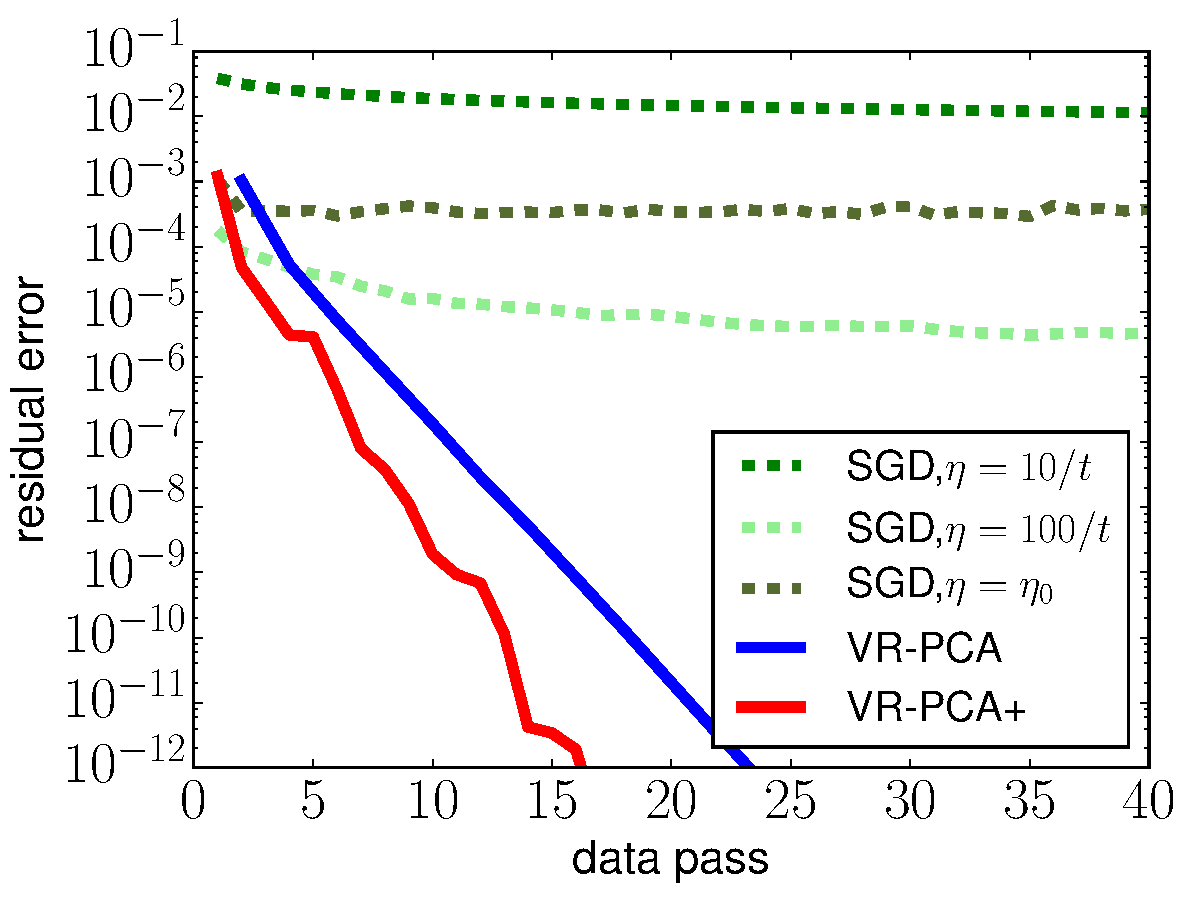
\includegraphics[width=0.5\columnwidth]{pca-4-mnist}\label{pca-4-mnist}}
\subfigure[cifar10, $k=4$]{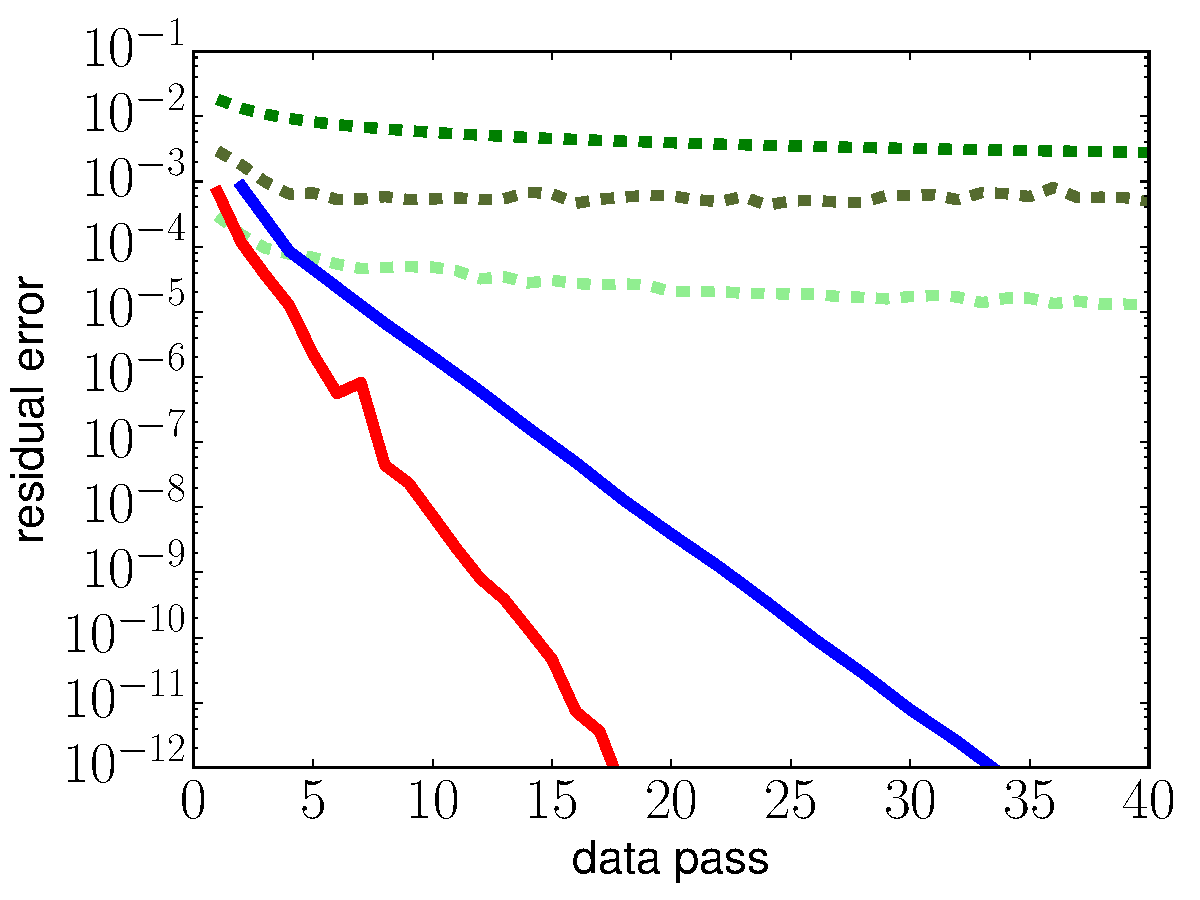
\includegraphics[width=0.5\columnwidth]{pca-4-cifar10}\label{pca-4-cifar10}}
\subfigure[mnist $k=6$]{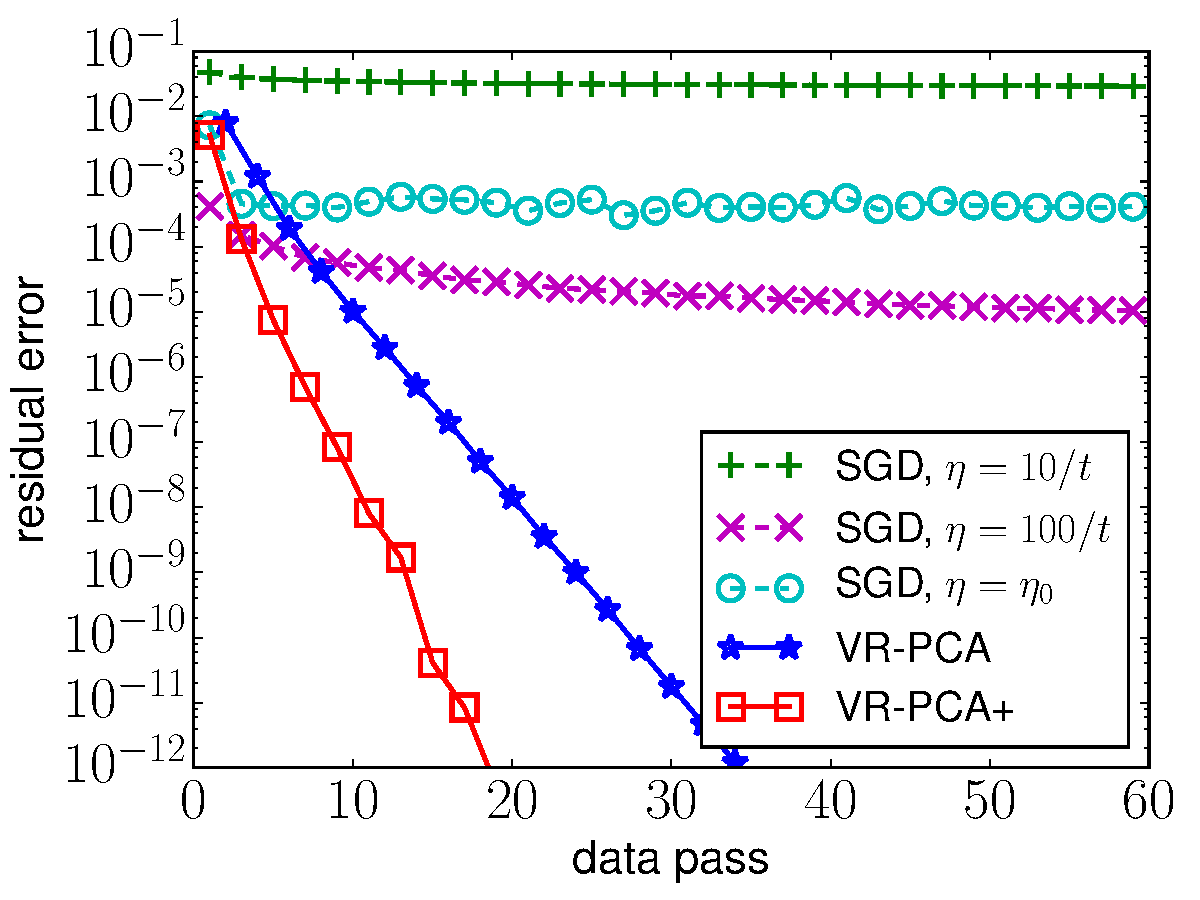
\includegraphics[width=0.5\columnwidth]{pca-6-mnist}\label{pca-6-mnist}}
\subfigure[cifar10 $k=6$]{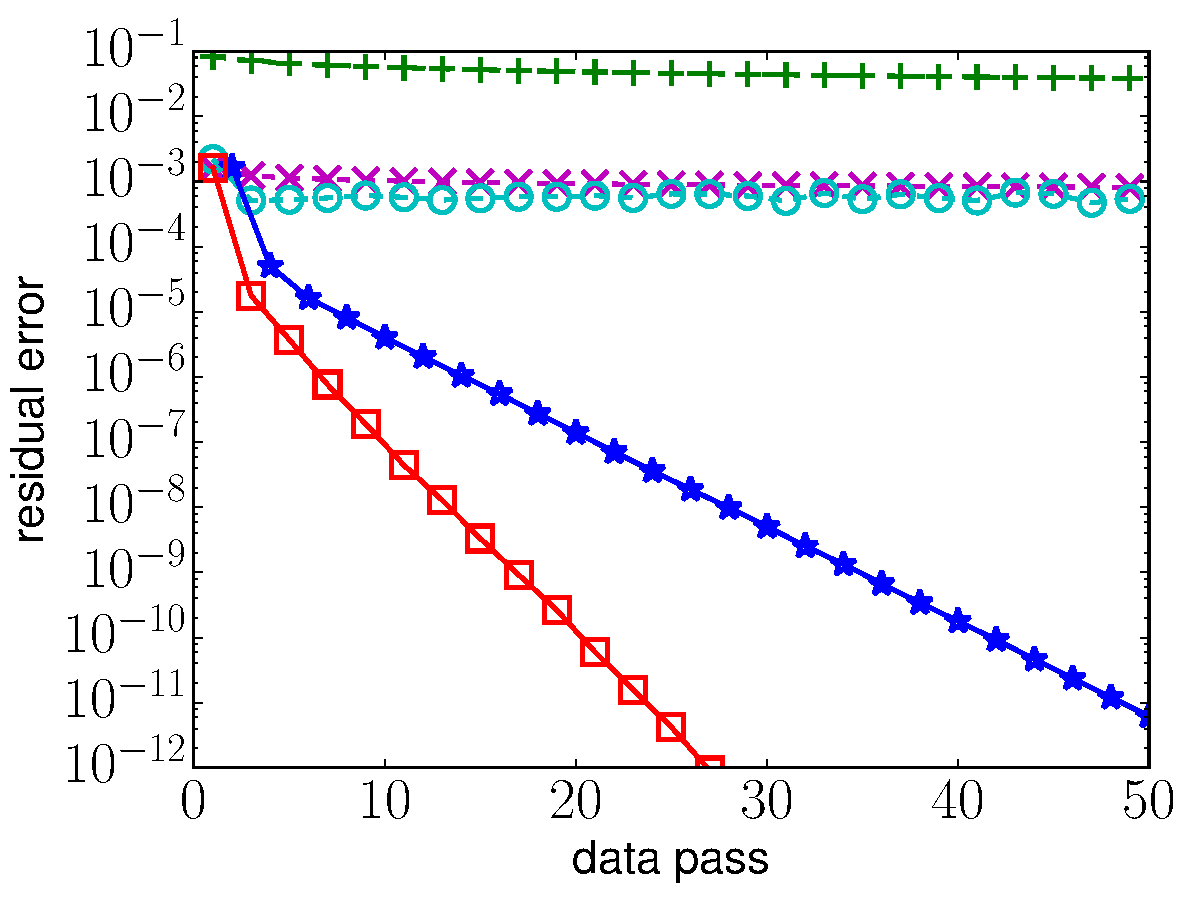
\includegraphics[width=0.5\columnwidth]{pca-6-cifar10}\label{pca-6-cifar10}}
%\caption{Generally, \textsc{aeSVRG} can automatically set an appropriate $m$ with different learning rates for the $l2$-regularized logistic regression on the dataset ijcnn1}
\caption{Generally, both VR-PCA and VR-PCA+ converge to a high precision and VR-PCA+ has a better performance.}
\label{pca}
\end{figure*}
 
 \begin{figure*}[ht]
\centering
\subfigure[mnist, $k=4$]{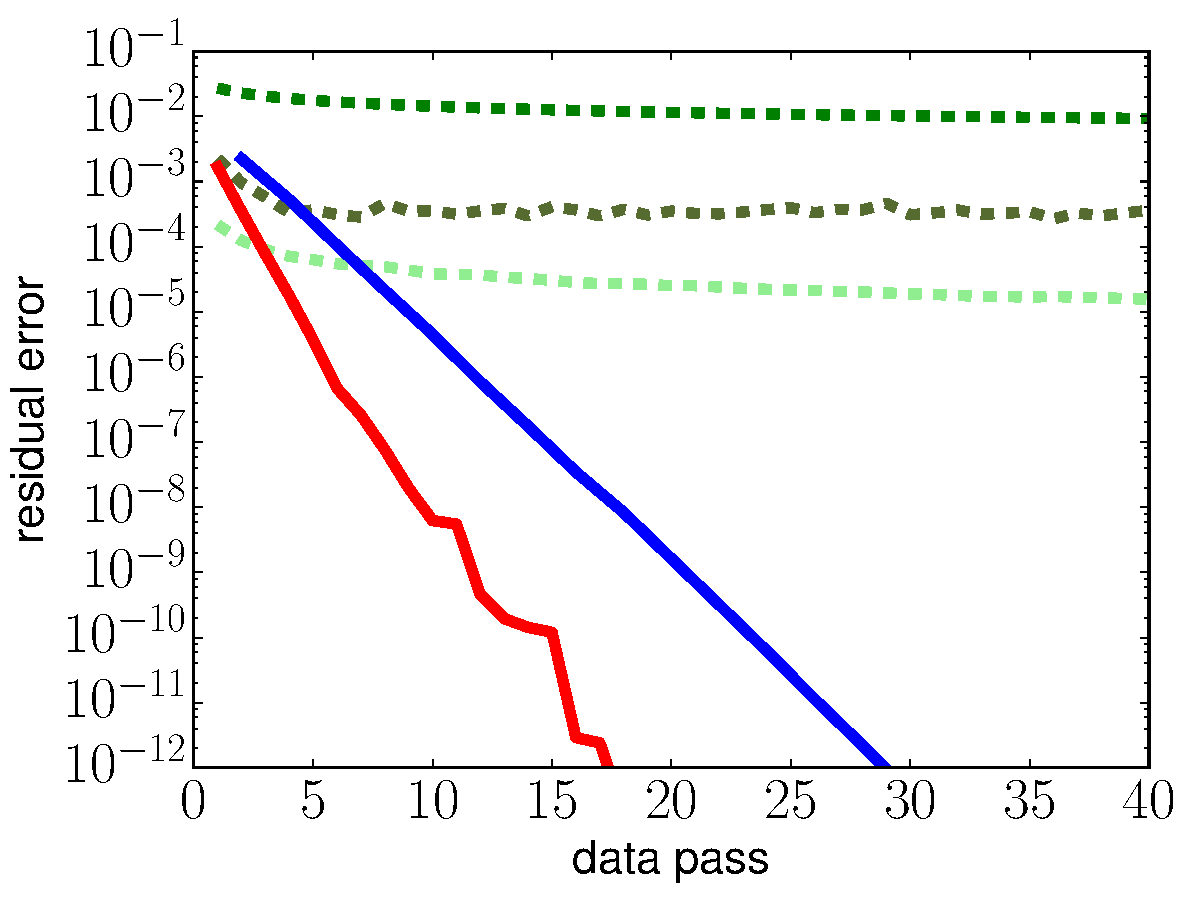
\includegraphics[width=0.5\columnwidth]{pls-4-mnist}\label{pls-4-mnist}}
\subfigure[cifar10, $k=4$]{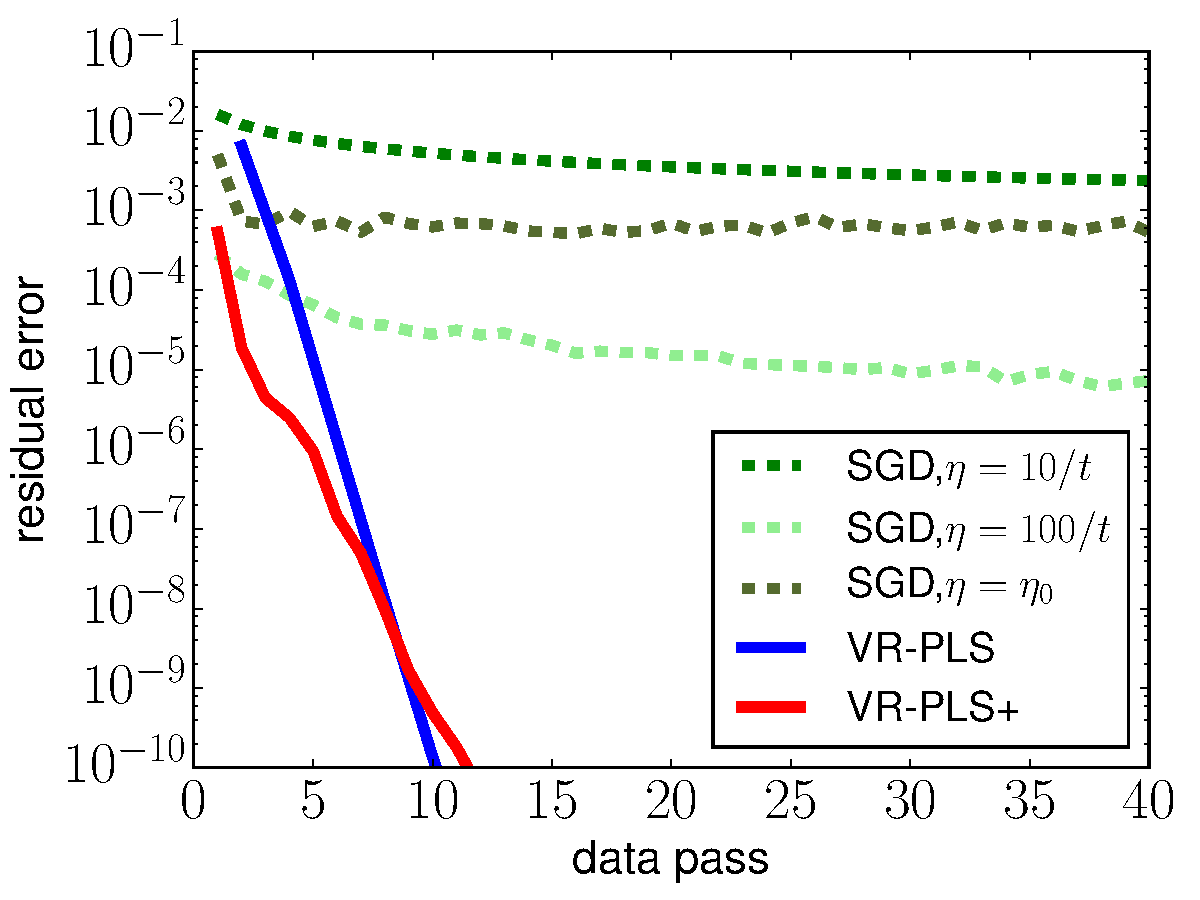
\includegraphics[width=0.5\columnwidth]{pls-4-cifar10}\label{pls-4-cifar10}}
\subfigure[mnist $k=6$]{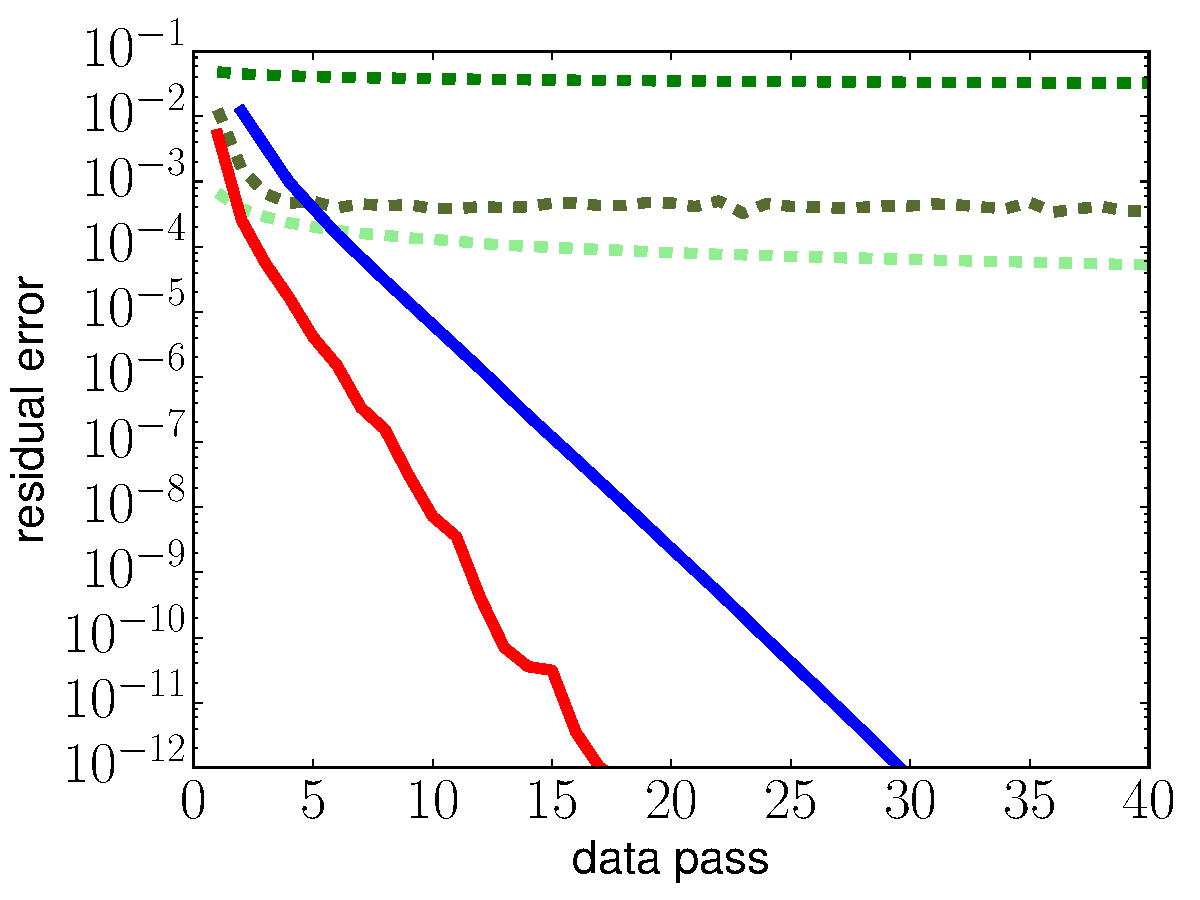
\includegraphics[width=0.5\columnwidth]{pls-6-mnist}\label{pls-6-mnist}}
\subfigure[cifar10 $k=6$]{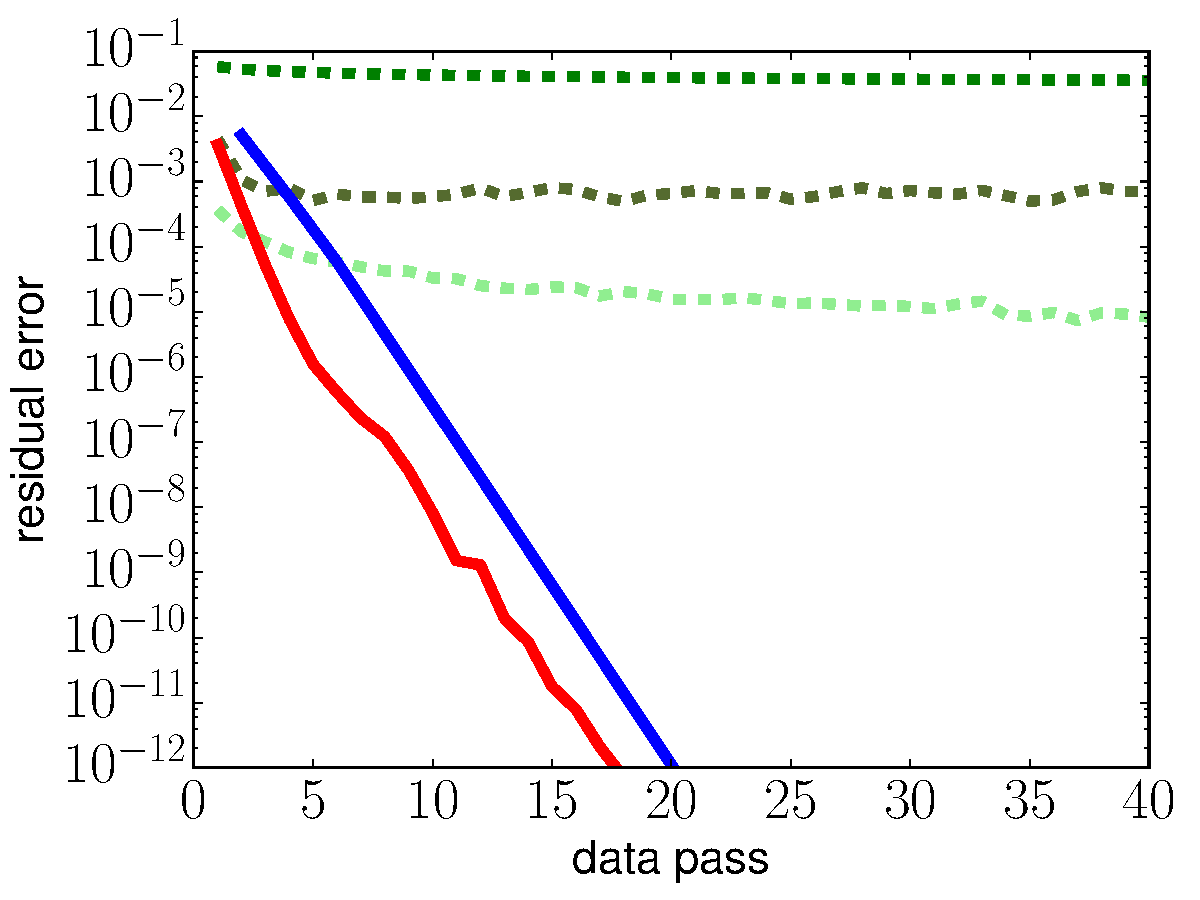
\includegraphics[width=0.5\columnwidth]{pls-6-cifar10}\label{pls-6-cifar10}}
%\caption{Generally, \textsc{aeSVRG} can automatically set an appropriate $m$ with different learning rates for the $l2$-regularized logistic regression on the dataset ijcnn1}
\caption{Generally, both VR-PLS and VR-PLS+ converge to a high precision and VR-PLS+ has a better performance in most cases.}
\label{pls}
\end{figure*}
 
 \begin{figure*}[ht]
\centering
\subfigure[mnist, $k=4$, pca]{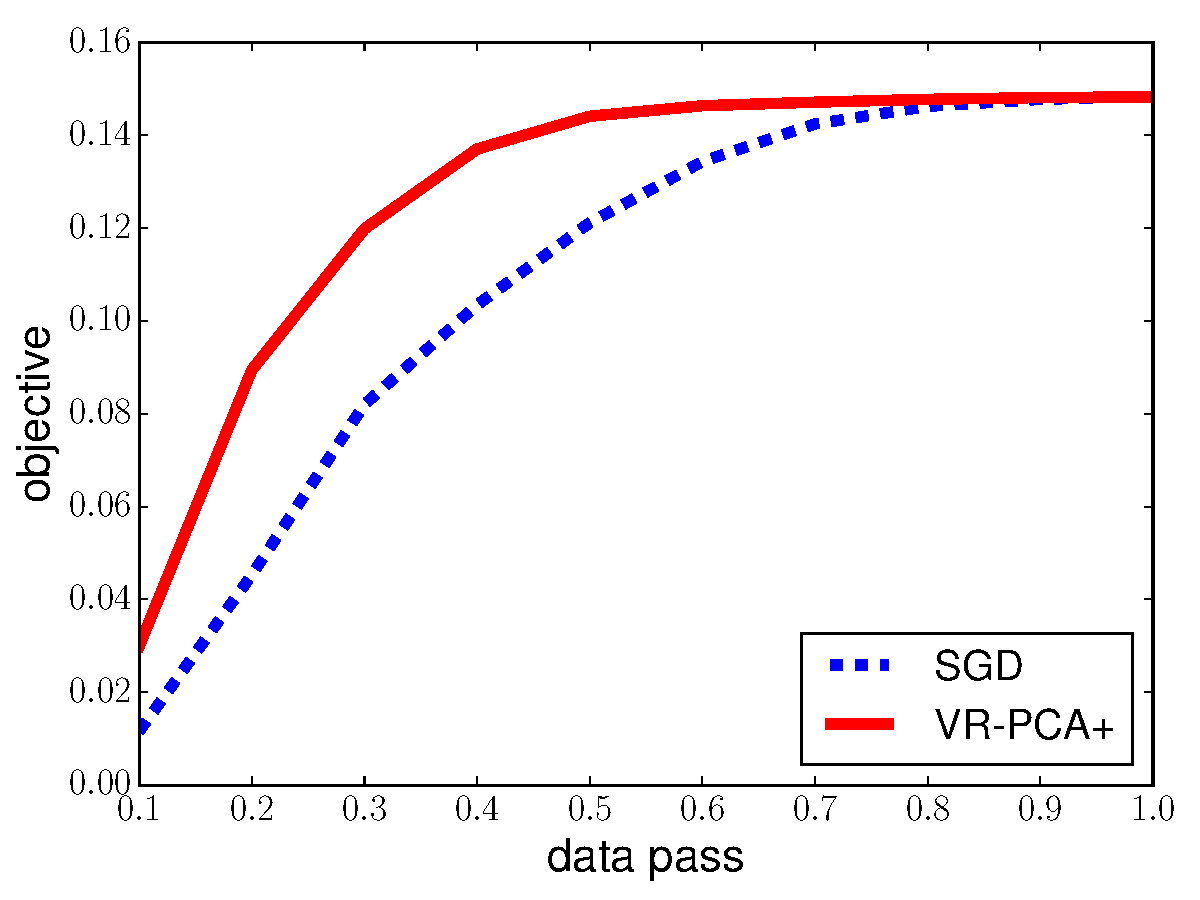
\includegraphics[width=0.5\columnwidth]{one-pca-4-mnist}\label{o-pca-4-mnist}}
\subfigure[mnist $k=6$, pca]{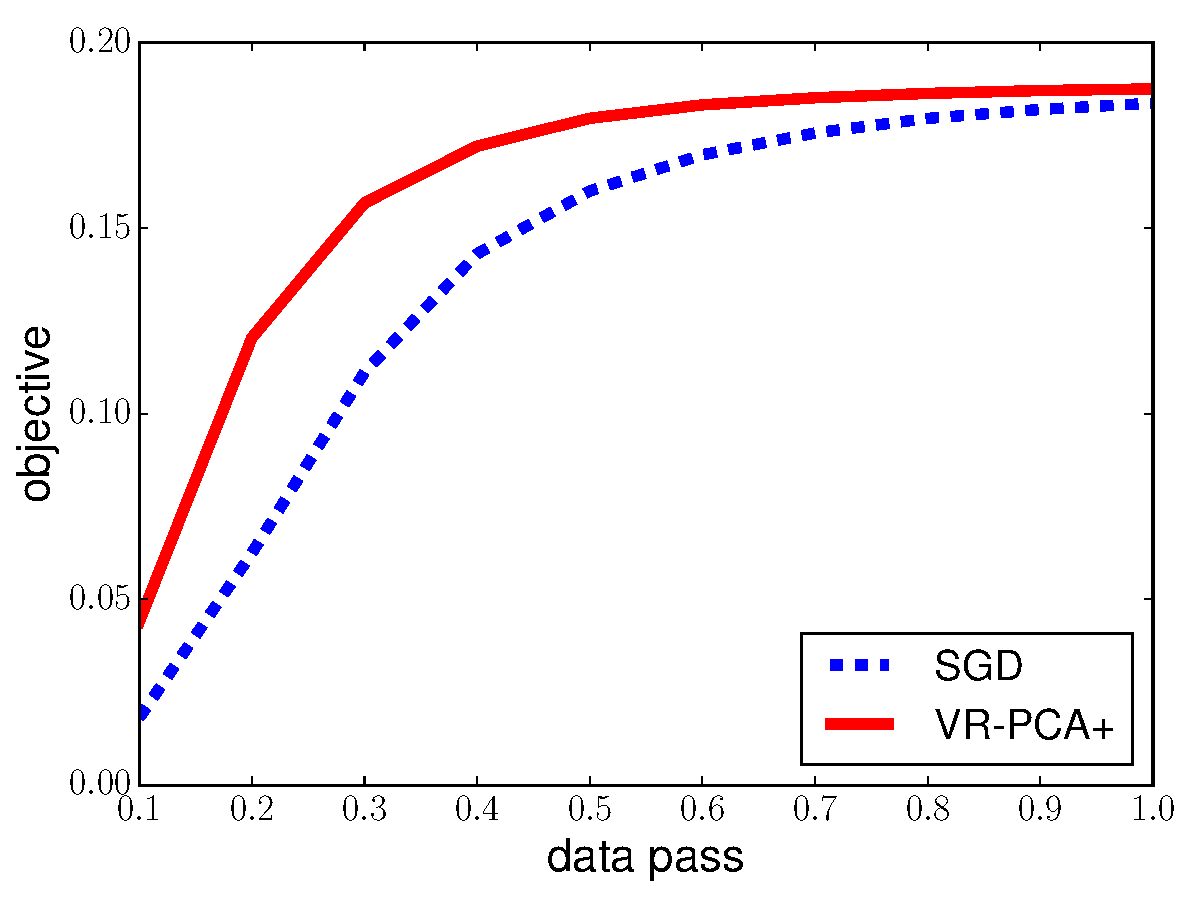
\includegraphics[width=0.5\columnwidth]{one-pca-6-mnist}\label{o-pca-6-mnist}}
\subfigure[cifar10, $k=4$, pls]{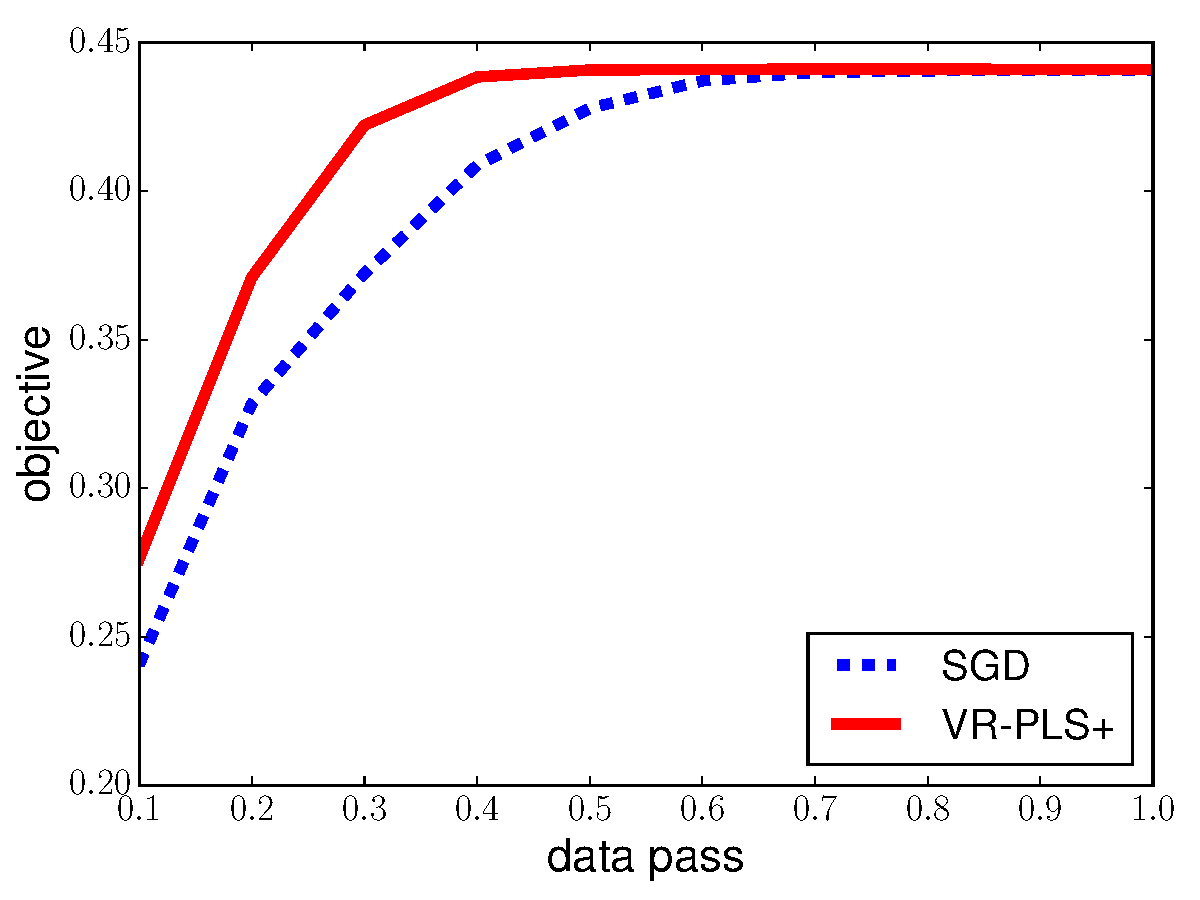
\includegraphics[width=0.5\columnwidth]{one-pls-4-cifar10}\label{o-pls-4-cifar10}}
\subfigure[cifar10 $k=6$, pls]{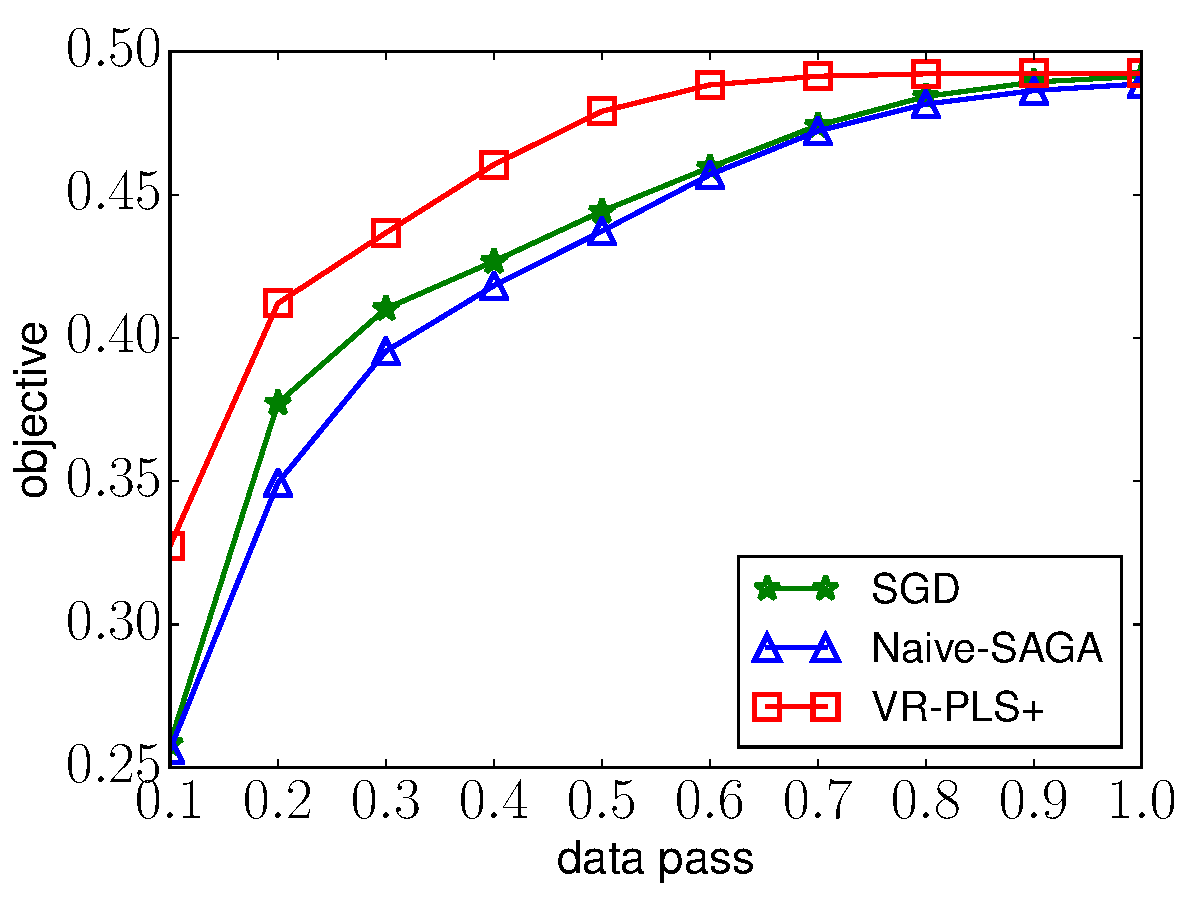
\includegraphics[width=0.5\columnwidth]{one-pls-6-cifar10}\label{o-pls-6-cifar10}}
\caption{Generally, VR-PCA(PLS)+ performs better than SGD in the first data pass.}
\label{one pass}
\end{figure*}

 \begin{figure*}[ht]
\centering
\subfigure[mnist, $pca$]{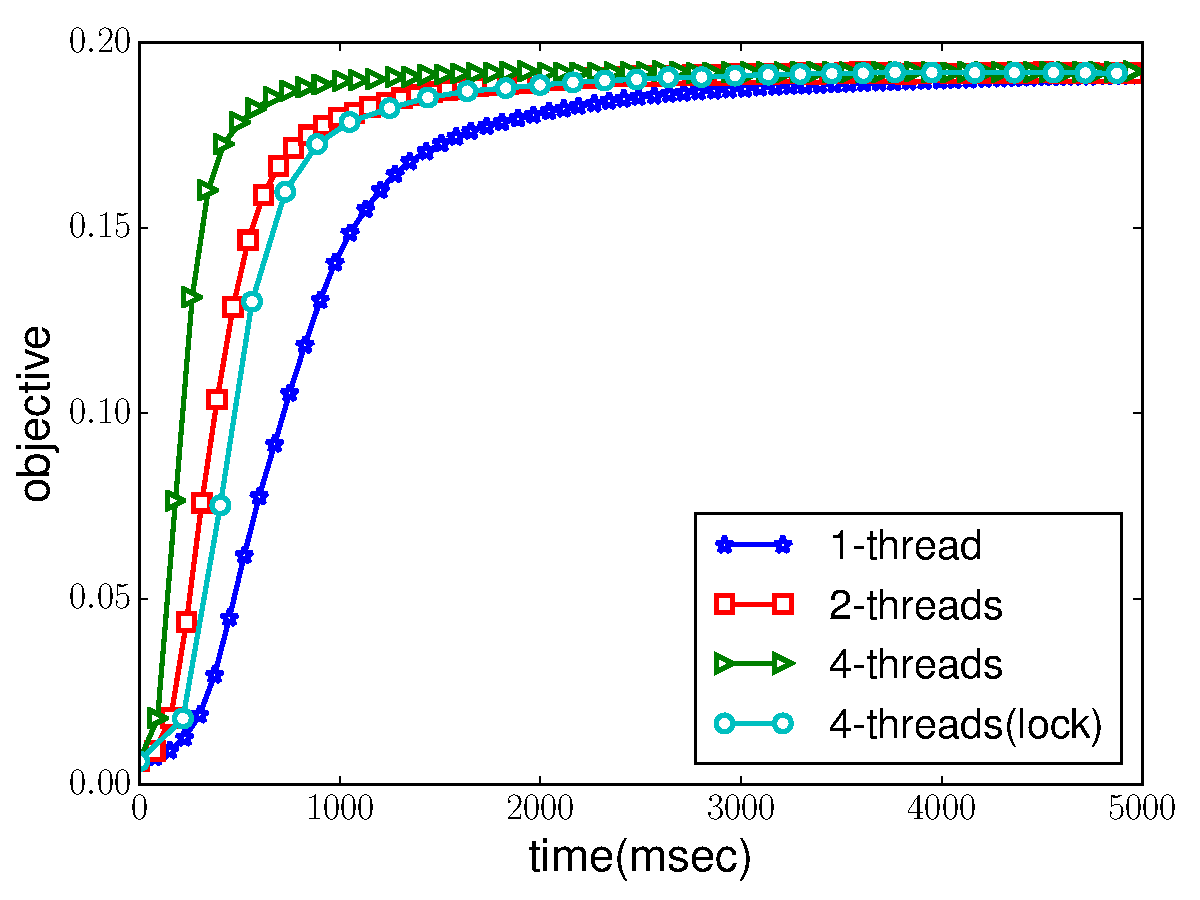
\includegraphics[width=0.5\columnwidth]{asgd-pca-mnist}\label{asgd-pca-mnist}}
\subfigure[cifar10, $pca$]{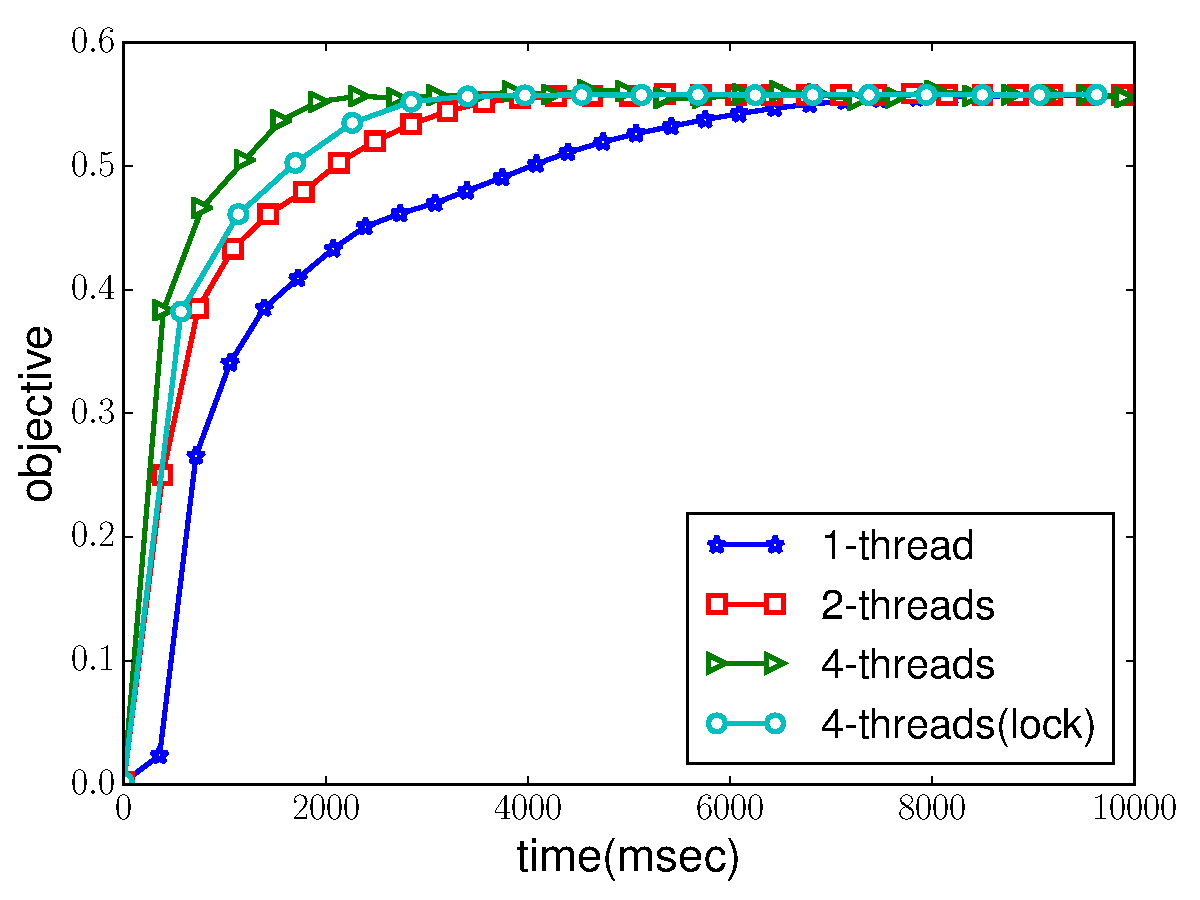
\includegraphics[width=0.5\columnwidth]{asgd-pca-cifar10}\label{asgd-pca-cifar10}}
\subfigure[mnist $pls$]{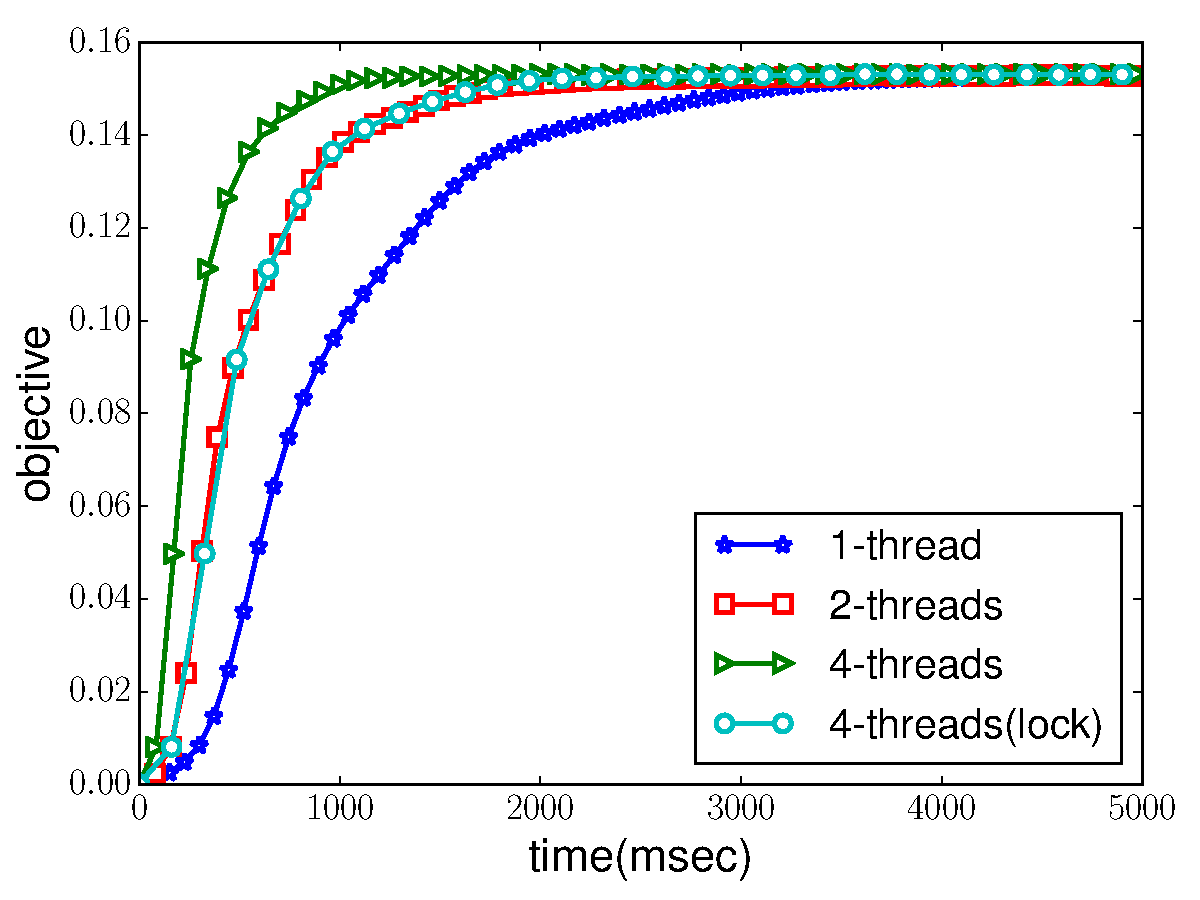
\includegraphics[width=0.5\columnwidth]{asgd-pls-mnist}\label{asgd-pls-mnist}}
\subfigure[cifar10 $pls$]{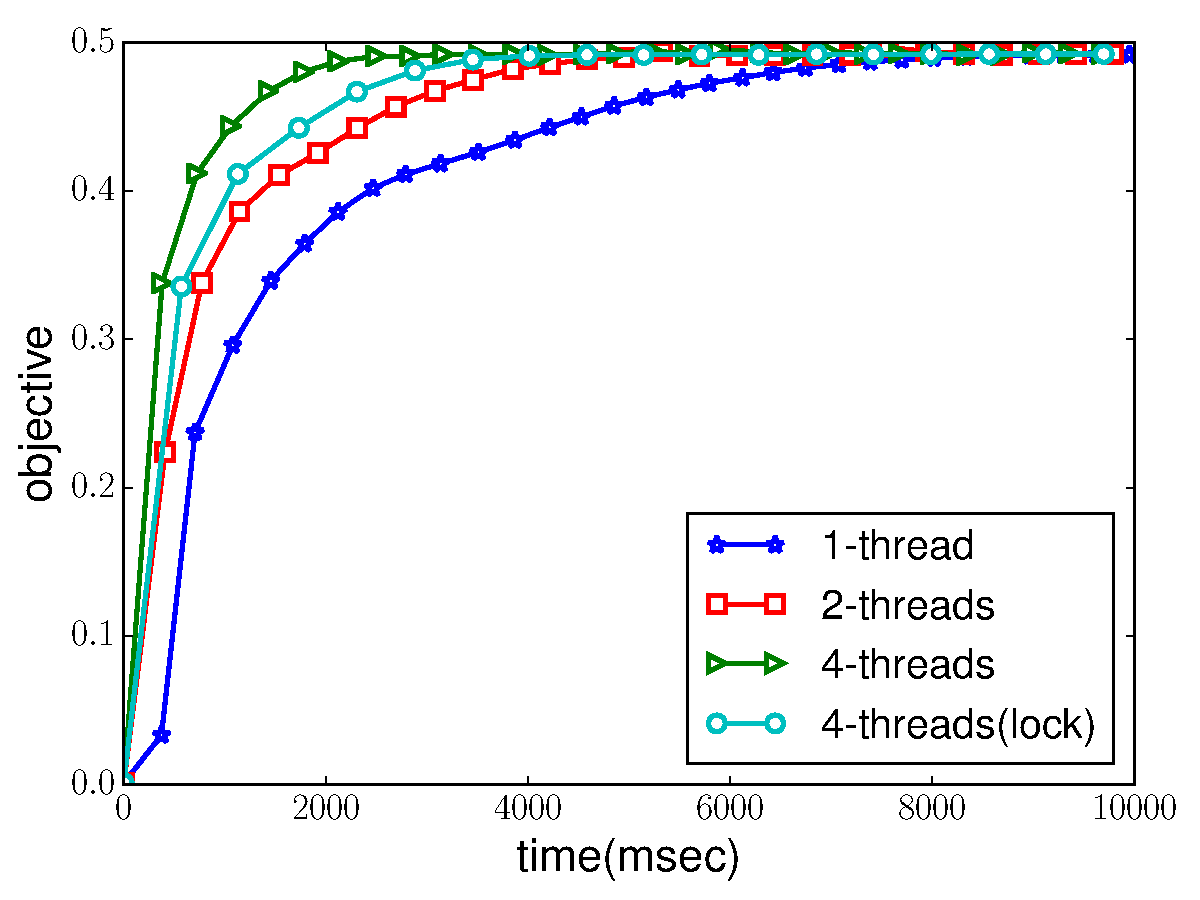
\includegraphics[width=0.5\columnwidth]{asgd-pls-cifar10}\label{asgd-pls-cifar10}}
\caption{Generally, asynchronous SGD for PCA(PLS) performs better with more threads. And the lock-free variant converges faster than lock variant.}
\label{asgd}
\end{figure*}


 
 \section{Numerical Experiments}
 \label{experiments}
 In this section, we present extensive experiments to demonstrate the performance of our proposed algorithms, i.e. VR-PLS and VR-PLS+. Our experiments include three parts, 
 In the first part, we run algorithms for several data passes to verify the performances of our proposed algorithms when high-precision is required.
 In the second part, we run algorithms for only one data pass to show the superior performances of VR-PCA+ and VR-PLS+ when computational overhead is limited.
 In the third part, we test asynchronous SGD for PCA and PLS with multi-threads.  
  Instead of parameters tuning, we heuristically set the epoch size $m$ of VR-PCA and VR-PLS as $n$ (the size of the dataset), and set the learning rate $\eta$ as recommended in [Shamir 2015]: $\eta_0 = \frac{1}{\gamma\sqrt{n}}$, where $\gamma = \frac{1}{n}\sum\limits_{i=1}^{n}{\Vert \mathbf{x}_i\Vert}^2$. Although this choice of $\eta_0$ is theoretically proved only for VR-PCA, we also find it suitable for other three algorithms in practice.
  %We performed experiments on both synthetic datasets and real world datasets. The synthetic datasets are generated through the following steps: Firstly, we construct a $d \times n$ matrix X according to a standard Gaussian distribution. Then we conduct SVD on it, $X = USV^{\top}$, set $S_{ii} = \lambda^{-i}$($\lambda$ is a number sightly larger than 1) and normalize S to one, then we obtain a new data matrix $\tilde{X} = U\tilde{S}V^{\top}$. After that, we let $\mathbf{x}_1 = R_{1}{U_1}^T\tilde{X}$ and $\mathbf{x}_2 = R_{2}{U_2}^T\tilde{X}$, where $U_1$ and $U_2$ are $d \times d_x$ and $d \times d_y$ random orthogonal matrices, $R_1$ and $R_2$ are random $d_x \times d_x$ and $d_y \times d_y$ random rotation matrices. In our experiments, we set $n = 10000, d = 1000, d_x=d_y=500$, and we set $\lambda$ as $1.2$ and $1.6$ to generate two different synthetic datasets. 
  We conducted experiments on the two famous datasets, MNIST and CIFAR-10. MINST dataset(LeCun et al., 1998) consists of $60,000$ handwritten digits from 0 to 9 and each instance is a $28 \times 28$ image. The CIFAR-10 dataset consists of $60,000$ color images of $32 \times 32$ in 10 classes and we just select the $50,000$ training examples. 
  For PCA experiments we directly use the datasets. For PLS experiments we split each pictures into left half part and right half part and generate a pair of dataset X and dataset Y. Therefore, for MNIST, $d_x = d_y = 392$ and for CIFAR-10, $d_x = d_y = 512$.
 All experiments include the preprocessing step, consisting of centering the data and dividing each coordinate by its standard deviation times the squared root of the dimension. 
 
 
 
 
 \subsection{Experiments for high-precision requirement}
 In this section we demonstrate the effectiveness and efficiency of our proposed algorithms. The evaluation criterion is the progress made on the objective as a function of iteration number, which is suitable for evaluating gradient optimization algorithms. 
 For comparison, we implemented the SGD algorithm, using several different initial step sizes with decaying strategy. We did not implement other sophisticated iterative algorithms mentioned in Section \ref{introduction} for the same reason with \citep{Shamir2015A}, as they are not directly comparable to the stochastic gradient algorithms due to inherent complexity per iteration and considerable memory requirement.
  The algorithms compared were initialized from the same random matrices. The results are displayed in figure \ref{pca} and figure \ref{pls}.
  In all figures, the x-axis represents the number of effective data passes (assuming 2 per epoch for VR-PCA and VR-PLS, 1 per epoch for VR-PCA+ and VR-PLS+), and the y-axis represent the residual, i.e., $tr(\hat{W}^{\top}X^{\top}X\hat{W}) - tr(W^{\top}X^{\top}XW)$ for PCA and $tr(\hat{U}^{\top}X^{\top}Y\hat{V}) - tr(U^{\top}X^{\top}YV)$ for PLS. Note the $X$,$Y$ are the data matrices, $\hat{W}$, $\hat{U}$, $\hat{V}$ are the optimal parameter matrices obtained by SVD, W, U, V are the matrices obtained so far. 
 From the figures we see that for different datasets and $k$, SGD algorithms appears to have a sub-linear convergence rate and fail to achieve a high-precision result, no matter which step strategy is applied.
In contrast, both VR-PCA(PLS) and VR-PCA(PLS)+ rapidly converge to an accuracy higher than $10^{-10}$, the main reason is that they have much lower variance than naive SGD algorithm. Besides, we also find the VR-PCA(PLS)+ have a better performance than VR-PCA(PLS) in most cases. It is not surprising since the SAGA-based algorithms do not require to compute the batch-gradient occasionally, which is time-consuming.
 
 \subsection{Experiments with limited time overhead}
 In this part we limit the computational cost within one data pass. Since VR-PCA(PLS) do not optimize the objective function in the first data pass, they were not experimented. Hence we only compare the VR-PCA(PLS)+ with SGD algorithm, setting the learning rate as $\eta_0$ for all experiments.
 The results are illustrated in figure \ref{one pass}.  Note that the x-axis still represents the number of data passes while the y-axis denotes the value of objective function. As we can see in figure \ref{one pass}, VR-PCA(PLS)+ always perform better than SGD algorithm, the main reason is that the variance reduced stochastic gradient of VR-PCA(PLS)+ is the combination of a stochastic gradient and a stale mini-batch gradient, which has a smaller variance than naive SGD.
 
 \subsection{Asynchronous SGD for PCA and PLS}
In this experiment, we compare asynchronous SGD for PCA and PLS with varying number of threads. 
We run the lock-free asynchronous SGD for 1, 2 and 4 threads. Besides, we also implement a lock variant and run it with 4 threads. Note the the evaluation criterion is the progress made on the objective as a function of time pass, thus the x-axis represents the time pass and y-axis represents the value of objective function. As we can see in Figure \ref{asgd}, the objective function converges faster with more threads, which demonstrates the effectiveness of asynchronism. Moreover, the lock-free variant performs better than lock variant, which is consistent with the primal SGD.
 


\section{Conclusion and Future Works}
\label{discussion}
Deterministic optimization algorithms for PCA and PLS suffer from unbearable computation cost in large-scale application, while stochastic algorithm is prohibitive from a high-accuracy solution. Thus it is natural to apply the variance reduced stochastic method to solve PCA and PLS. In this paper, we review the SVRG-based algorithm for PCA, i.e., VR-PCA, and extend it to PLS. Besides, we propose the novel
SAGA-based algorithms, which performs better than SVRG-based algorithms and apply to time limited conditions. Moreover, since stochastic gradient algorithms are inherently suitable for asynchronism, we explore an implement of asynchronous SGD for PCA and PLS. 
Although we have not rigorously conducted convergence analysis on the proposed algorithms, all of them prove to be experimentally efficient.
We leave the following future works: (1) Prove the convergence of proposed algorithms theoretically. (2) Research the asynchronous variants of VR-PCA(PLS) and VR-PCA(PLS)+. (3) Explore other constrained objective functions which can be optimized through stochastic power methods and its variance reduced variants.



\section*{Acknowledgment}






%\bibliographystyle{plain}
\bibliographystyle{unsrt}
\bibliography{reference}


% that's all folks
\end{document}


